\documentclass[11pt]{article}
\usepackage[utf8]{inputenc}
\usepackage[T1]{fontenc}
\usepackage{geometry}
\usepackage{hyperref}
\usepackage{enumitem}
\usepackage{tikz}
\usetikzlibrary{positioning}

\geometry{margin=1in}

\title{BS Portfolio 01 MealPlanner}
\author{
  \textit{[Author Name 1]} (\textit{[Matriculation Number]})\\
  \textit{[Author Name 2]} (\textit{[Matriculation Number]})
}
\date{October 27, 2025}

\begin{document}

\maketitle

\section{Project Overview}

\textbf{Elevator Pitch:} Food prices for similar products vary dramatically, often by several multiples. 
MealPlanner helps people reach their fitness and nutrition goals on a budget by showing them which foods and meals give them the best value for their money based on what they want to achieve, whether thats losing weight, building muscle, or both.

\textbf{Persona 1.} 23 year old student
Problem: He weighs 90kg and wants to increase his muscle mass. However, as a student, he has a tight budget for food. 
What is the most cost-effective way to get enough calories and protein without breaking the bank?

Solution: MealPlanner allows users to filter foods by:
\begin{itemize}[noitemsep]
  \item Price per 100g protein
  \item Price per 1000 calories
\end{itemize}
This helps find affordable options that meet his nutritional needs.

\textbf{Persona 2.} 35 year old working professional
Problem: She wants to lose weight but has a busy schedule and limited time for meal prep. What are the best meal options that are both healthy and quick to prepare?

Solution: Meal Planner enables her to create and search for dishes based on:
\begin{itemize}[noitemsep]
  \item Calories per serving
  \item Caloric density (calories per gram)
  \item Preparation time
\end{itemize}
This allows her to find meals that fit her weight loss goals and time constraints.


\textbf{What We Built.} Our system manages four main components: food items, dishes, users, and shopping carts. Users can add food items and create Dishes with them. Once created the system automatically calculates nutritional values and costs. The user then, can filter those dishes by their nutritional value, cost or the required time to prepare them. Once users find a suitable dish, they can automatically add all ingredients (with the corresponding quantity) to their shopping cart for convenient purchasing.



\textbf{Scope Limitations.} The first increment explicitly excludes allergen/micronutrient modeling and differentiation between coach/client roles – all users have the same capabilities to create food items and dishes as well as filter and purchase them. Unit differentiation (pieces, liters vs. grams) is also excluded to keep the deliverable focused.

\section{Domain Model}

The following domain model describes the main objects of the system. 
It shows important entities, their attributes, and how they are connected. 
The system focuses on users, food items, dishes, and a shopping cart for buying ingredients.

\begin{figure}[h]
  \centering
  \resizebox{0.9\linewidth}{!}{%
  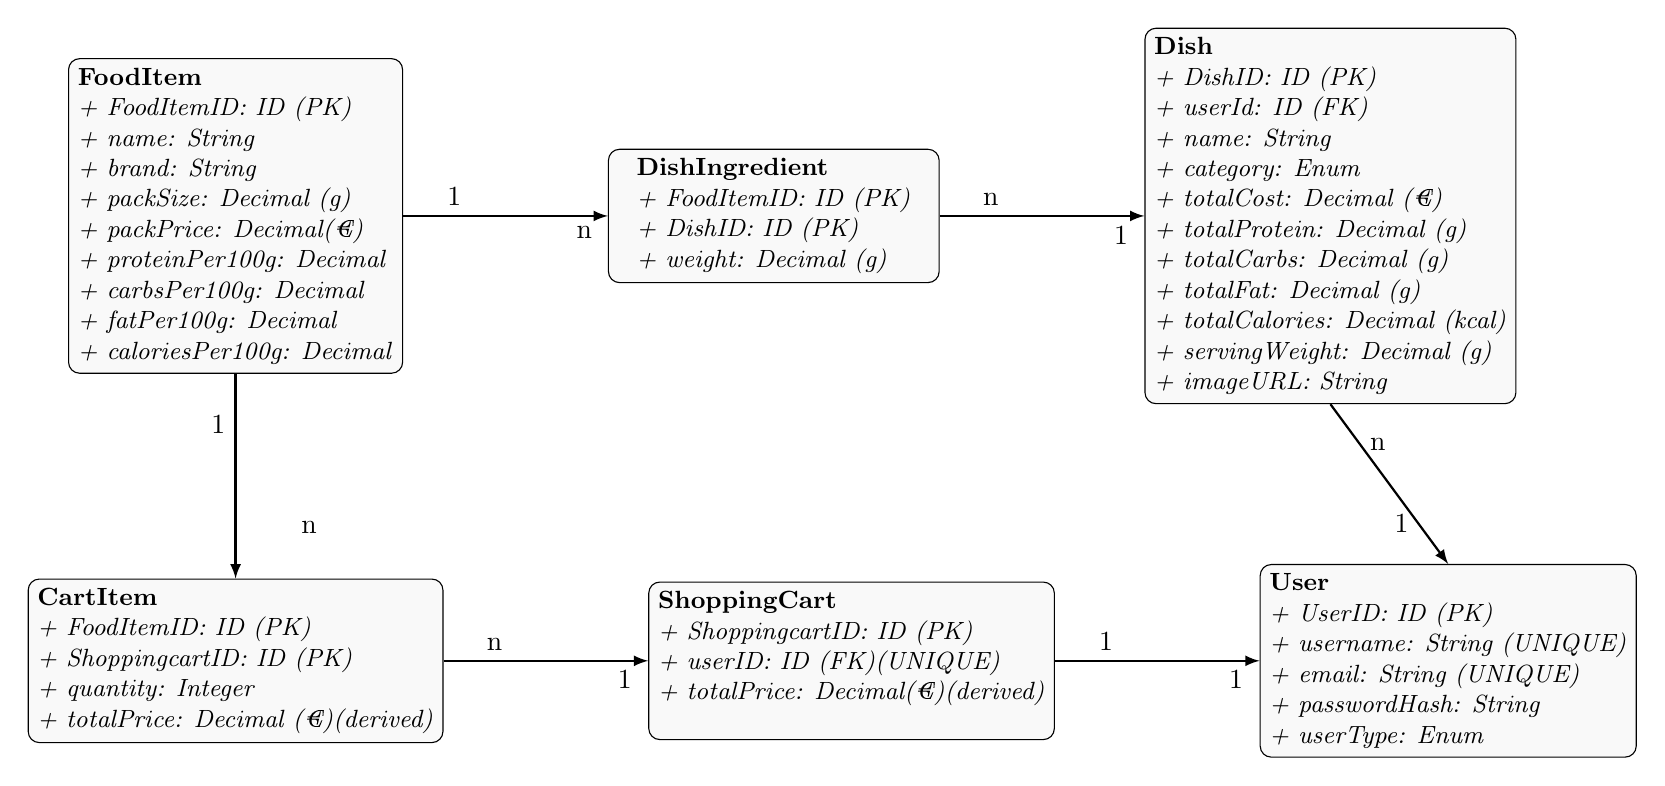
\begin{tikzpicture}[
    class/.style={rectangle, draw, rounded corners, minimum width=4.2cm, align=left, font=\small, fill=gray!5},
    relation/.style={-latex, thick},
    node distance=2.6cm
  ]

    % Row 1: FoodItem, DishIngredient, Dish
    \node[class] (food) {
      \textbf{FoodItem}\\
      \textit{+ FoodItemID: ID (PK)}\\
      \textit{+ name: String}\\
      \textit{+ brand: String}\\
      \textit{+ packSize: Decimal (g)}\\
      \textit{+ packPrice: Decimal(€)}\\
      \textit{+ proteinPer100g: Decimal}\\
      \textit{+ carbsPer100g: Decimal}\\
      \textit{+ fatPer100g: Decimal}\\
      \textit{+ caloriesPer100g: Decimal}
    };

    \node[class, right=of food] (dishIng) {
      \textbf{DishIngredient}\\
      \textit{+ FoodItemID: ID (PK)}\\
      \textit{+ DishID: ID (PK)}\\
      \textit{+ weight: Decimal (g)}
    };

    \node[class, right=of dishIng] (dish) {
      \textbf{Dish}\\
      \textit{+ DishID: ID (PK)}\\
      \textit{+ userId: ID (FK)}\\
      \textit{+ name: String}\\
      \textit{+ category: Enum}\\
      \textit{+ totalCost: Decimal (€)}\\
      \textit{+ totalProtein: Decimal (g)}\\
      \textit{+ totalCarbs: Decimal (g)}\\
      \textit{+ totalFat: Decimal (g)}\\
      \textit{+ totalCalories: Decimal (kcal)}\\
      \textit{+ servingWeight: Decimal (g)}\\
      \textit{+ imageURL: String}
    };

    % Row 2: CartItem, ShoppingCart, User
    \node[class, below=of food] (cartItem) {
      \textbf{CartItem}\\
      \textit{+ FoodItemID: ID (PK)}\\
      \textit{+ ShoppingcartID: ID (PK)}\\
      \textit{+ quantity: Integer}\\
      \textit{+ totalPrice: Decimal (€)(derived)}
    };

    \node[class, right=of cartItem] (cart) {
      \textbf{ShoppingCart}\\
      \textit{+ ShoppingcartID: ID (PK)}\\
      \textit{+ userID: ID (FK)(UNIQUE)}\\
      \textit{+ totalPrice: Decimal(€)(derived)}\\
    };

    \node[class, right=of cart] (user) {
      \textbf{User}\\
      \textit{+ UserID: ID (PK)}\\
      \textit{+ username: String (UNIQUE)}\\
      \textit{+ email: String (UNIQUE)}\\
      \textit{+ passwordHash: String}\\
      \textit{+ userType: Enum}
    };

    % Relations
    \draw[relation] (food) -- node[near start, above]{1} node[near end, below]{\quad\quad n} (dishIng);
    \draw[relation] (dishIng) -- node[near start, above]{n} node[near end, below]{\quad\quad 1} (dish);

    \draw[relation] (food) -- node[near start, left]{1} node[near end, right]{\quad\quad n} (cartItem);
    \draw[relation] (cartItem) -- node[near start, above]{n} node[near end, below]{\quad\quad 1} (cart);
    \draw[relation] (cart) -- node[near start, above]{1} node[near end, below]{\quad\quad 1} (user);
    % Vertical from dish bottom to user's top (north)
    \draw[relation] (dish.south) -- node[near start, right]{n} node[near end, left]{1} (user.north);
  \end{tikzpicture}%
  }
  \caption{UML class diagram of the Meal Planner domain.}
  \label{fig:uml}
\end{figure}

\subsection*{Main Entities}

\paragraph{FoodItem} represents a food product in a store. 
It includes nutritional information such as protein, carbohydrates, fat and calories per 100g, and also the pack size and price. 
A food item can be used in many dishes and can also appear many times in shopping carts.

\paragraph{DishIngredient} connects a \textit{Dish} with a \textit{FoodItem}.
It stores how many grams of the food item are used in the dish.
This creates a many-to-many relationship between dishes and food items.

\paragraph{Dish} is a recipe created by a user. 
The \textit{category} is an enum that stores if the dish is breakfast, lunch, dinner, dessert, snack or something else.
It also saves the 
\textit{total cost} in euros, 
\textit{total protein}, 
\textit{total carbohydrates}, 
\textit{total fat}, 
\textit{total calories}, 
and the \textit{serving weight} in grams.
A dish can also have an optional \textit{image link} to upload a photo of the Dish.

\paragraph{CartItem} connects a \textit{FoodItem} with a \textit{ShoppingCart}.
It stores the \textit{quantity} of the food item.
The \textit{total price} for the item is calculated from the quantity.

\paragraph{ShoppingCart} belongs to one user.
It can contain many \textit{CartItem} objects.
The \textit{total price} of the shopping cart is calculated from all items inside it.

\paragraph{User} represents a registered person in the system. 
Each user has a unique \textit{username} and \textit{email}. 
The \textit{password} is saved as a hash for security.
The \textit{userType} is an enum that stores the user's goal, such as building muscle, losing weight, gaining weight or living a healthier lifestyle.
A user can create many dishes, but each user has only one shopping cart.


\subsection*{Rules and Constraints}

\begin{itemize}
    \item Each username and email must be unique.
    \item A user can only have one shopping cart at the same time.
    \item Nutritional values and prices cannot be negative.
    \item Quantity in a cart and weight in a dish must be greater than 0.
    \item Total calories, total cost, and other totals are calculated automatically.
\end{itemize}

\subsection*{Example Records}

\paragraph{Example FoodItem}
\begin{verbatim}
FoodItemID = 101
name = "Oats"
brand = "BioFarm"
packSize = 1000 g
packPrice = 2.79 €
proteinPer100g = 12 g
carbsPer100g = 60 g
fatPer100g = 7 g
caloriesPer100g = 370 kcal
\end{verbatim}

\paragraph{Example Dish}
\begin{verbatim}
DishID = 22
userID = 5
name = "Protein Oatmeal"
category = Breakfast
servingWeight = 350 g
totalCalories = 520 kcal
totalProtein = 32 g
totalCost = 1.10 €
\end{verbatim}

These examples show how real data can appear in the system.
The domain model gives a clear and structured overview of users, food items, dishes, and shopping carts.
It supports the calculation of nutrition values and costs, the management of ingredients, and the planning of meals and shopping.
In this way, the model helps to create an organized and efficient system for healthy eating and meal preparation.

\section{Use Cases}

The backend covers six core use cases. Each use case follows a clear structure with preconditions, a main flow, alternate/failure flows, postconditions, and acceptance criteria.

\subsection*{UC01 -- Register Food Item (Must)}
\textbf{Primary Actor:} User\\
\textbf{Goal (User Story):} ``As a user, I want to register an ingredient with correct nutrition and pricing so later calculations are reliable.''\\
\textbf{Preconditions:} The name is unique; pack size and price are positive; macro values per 100\,g are within sensible ranges; brand is optional.\\
\textbf{Main Success Scenario:}
\begin{enumerate}[label=\arabic*.]
  \item The actor submits \texttt{POST /food-items} with name, optional brand, pack size (g), pack price, and protein/carbs/fat/calories per 100\,g.
  \item The service validates values, rounds to two decimals, and computes helper metrics (e.g., price per 100\,g).
  \item The database stores the \texttt{FoodItem} with timestamps.
  \item The API returns \texttt{201 Created} with the id and the saved record.
\end{enumerate}
\textbf{Alternate / Failure Flows:}
\begin{enumerate}[label=\arabic*F.]
  \item Duplicate name $\rightarrow$ \texttt{409 Conflict} with instructions to choose a distinct name.
  \item Out-of-range or negative values $\rightarrow$ \texttt{400 Bad Request} with details.
\end{enumerate}
\textbf{Postconditions:} The \texttt{FoodItem} is stored in a standard format and can be used to compose dishes.\\
\textbf{Acceptance Criteria:}
\begin{itemize}[noitemsep]
  \item Numeric fields are stored with two decimals; invalid values are rejected with clear messages.
  \item Derived metrics (e.g., price per 100\,g) are correct to two decimals.
\end{itemize}

\subsection*{UC02 -- Compose Dish (Must)}
\textbf{Primary Actor:} Nutrition planner\\
\textbf{Goal (User Story):} ``As a planner, I want to create a dish from precise ingredient weights so totals are computed automatically.''\\
\textbf{Preconditions:} At least one \texttt{FoodItem} exists; each ingredient grams value is > 0; each \texttt{FoodItem} appears at most once in the dish.\\
\textbf{Main Success Scenario:}
\begin{enumerate}[label=\arabic*.]
  \item The actor calls \texttt{POST /dishes} with name, servings, and an ingredients array of \{\texttt{foodItemId}, \texttt{grams}\}.
  \item The application service loads the referenced \texttt{FoodItem}s and computes total cost and macronutrients; per-serving values use \texttt{servingGrams}.
  \item The transaction persists \texttt{Dish} and \texttt{DishIngredient} entities atomically.
  \item The API returns \texttt{201 Created} with computed totals and a version number for concurrency.
\end{enumerate}
\textbf{Alternate / Failure Flows:}
\begin{enumerate}[label=\arabic*F.]
  \item Unknown \texttt{foodItemId} $\rightarrow$ \texttt{404 Not Found}.
  \item Duplicate \texttt{foodItemId} in the payload $\rightarrow$ \texttt{400 Bad Request} with guidance to merge grams.
  \item Ingredient grams $\leq 0$ $\rightarrow$ \texttt{400 Bad Request} with validation details.
\end{enumerate}
\textbf{Postconditions:} The dish is stored with correct totals and can be listed and adjusted.\\
\textbf{Acceptance Criteria:}
\begin{itemize}[noitemsep]
  \item Calculated totals equal the sum of ingredient contributions within rounding tolerance.
  \item Saved and fetched representations match, including totals and per-serving values.
\end{itemize}

\subsection*{UC03 -- Adjust Dish Composition (Should)}
\textbf{Primary Actor:} Nutrition planner\\
\textbf{Goal (User Story):} ``As a planner, I want to adjust ingredient weights so that cost and nutrition metrics remain accurate over time.''\\
\textbf{Preconditions:} The dish exists and currently references at least one ingredient.\\
\textbf{Main Success Scenario:}
\begin{enumerate}[label=\arabic*.]
  \item The actor uses sub-resources to modify composition:
    \begin{itemize}[noitemsep]
      \item Add: \texttt{POST /dishes/\{dishId\}/ingredients} with \{\texttt{foodItemId}, \texttt{grams}\}.
      \item Update: \texttt{PATCH /dishes/\{dishId\}/ingredients/\{dishIngredientId\}} with \{\texttt{grams}\}.
      \item Remove: \texttt{DELETE /dishes/\{dishId\}/ingredients/\{dishIngredientId\}}.
    \end{itemize}
  \item The domain validates all changes and recomputes totals, per-serving metrics, and derived rankings.
  \item The persistence layer commits in a single transaction and updates timestamps.
  \item The API returns the refreshed \texttt{Dish} with an incremented version.
\end{enumerate}
\textbf{Alternate / Failure Flows:}
\begin{enumerate}[label=\arabic*F.]
  \item Concurrent modification $\rightarrow$ \texttt{409 Conflict} with retry guidance.
  \item Removing all ingredients $\rightarrow$ \texttt{400 Bad Request} with ``Dish must contain at least one ingredient.''
\end{enumerate}
\textbf{Postconditions:} The dish reflects updated totals and remains consistent for listing and ranking.\\
\textbf{Acceptance Criteria:}
\begin{itemize}[noitemsep]
  \item Per-serving calculations update consistently after each modification.
  \item Versioning prevents overwrites and clearly signals conflicts.
\end{itemize}

\subsection*{UC04 -- Add Dish to Shopping Cart (Should)}
\textbf{Primary Actor:} Shopper preparing groceries\\
\textbf{Goal (User Story):} ``As a shopper, I want to add a whole dish to my shopping cart so that all its ingredients are added in the correct quantities automatically.''\\
\textbf{Preconditions:} The target \texttt{Dish} exists; an active shopping cart exists (or is created implicitly); \texttt{servingsMultiplier} is a positive integer.\\
\textbf{Main Success Scenario:}
\begin{enumerate}[label=\arabic*.]
  \item The actor calls \texttt{POST /shopping-carts/\{cartId\}/items/from-dish} with \{\texttt{dishId}, optional \texttt{servingsMultiplier}=1\}.
  \item The application service loads the dish and its \texttt{DishIngredient}s.
  \item For each ingredient, the service creates or increments a \texttt{CartItem} for the \texttt{foodItemId} with grams = \texttt{ingredient.grams} \(\times\) \texttt{servingsMultiplier}.
  \item The transaction persists all item changes and returns the updated cart state.
\end{enumerate}
\textbf{Alternate / Failure Flows:}
\begin{enumerate}[label=\arabic*F.]
  \item Unknown \texttt{dishId} or \texttt{cartId} $\rightarrow$ \texttt{404 Not Found}.
  \item Non-positive \texttt{servingsMultiplier} $\rightarrow$ \texttt{400 Bad Request} with validation details.
  \item Concurrent write to the same cart $\rightarrow$ \texttt{409 Conflict}; ask the user to retry.
\end{enumerate}
\textbf{Postconditions:} The shopping cart contains one item per \texttt{FoodItem} in the dish; grams are merged into existing items instead of duplicating lines.\\
\textbf{Acceptance Criteria:}
\begin{itemize}[noitemsep]
  \item Adding a dish creates or increments per-\texttt{FoodItem} items by \(\texttt{ingredient.grams} \times \texttt{servingsMultiplier}\).
  \item Re-adding the same dish with \texttt{servings = n} increases the same items cumulatively; no duplicate rows are created.
  \item When two dishes share a \texttt{FoodItem}, the cart reflects the summed grams across both additions.
\end{itemize}

\subsection*{UC05 -- Filter and Rank Food Items (Must)}
\textbf{Primary Actor:} Shopper or nutrition planner\\
\textbf{Goal (User Story):} ``As a user, I want to search, filter, and sort food items by cost and nutrition so that I can identify the best options for my goals and budget.''\\
\textbf{Preconditions:} At least one \texttt{FoodItem} exists with valid derived metrics.\\
\textbf{Main Success Scenario:}
\begin{enumerate}[label=\arabic*.]
  \item The actor calls \texttt{GET /food-items} with query parameters for filtering (e.g., min/max protein per 100\,g) and sorting (e.g., price per 100\,g protein).
  \item The application service builds a database query that uses derived metrics consistently.
  \item The API returns a paginated list including the requested sort order and summary fields.
\end{enumerate}
\textbf{Alternate / Failure Flows:}
\begin{enumerate}[label=\arabic*F.]
  \item No matching items $\rightarrow$ \texttt{200 OK} with an empty array.
  \item Unsupported filter or sort parameter $\rightarrow$ \texttt{400 Bad Request} listing allowed fields and formats.
\end{enumerate}
\textbf{Postconditions:} The actor receives a consistently ordered list of food items aligned to their constraints.\\
\textbf{Acceptance Criteria:}
\begin{itemize}[noitemsep]
  \item Sorting by price-per-protein and other metrics is stable and repeatable.
  \item Pagination metadata and caching headers are present and correct.
\end{itemize}

\subsection*{UC06 -- Cart Summary and Pack Estimates (Should)}
\textbf{Primary Actor:} Shopper preparing purchases\\
\textbf{Goal (User Story):} ``As a shopper, I want a consolidated shopping cart summary with estimated packs and total cost so that I can purchase the right amounts efficiently.''\\
\textbf{Preconditions:} The shopping cart exists and contains one or more items; each referenced \texttt{FoodItem} has a known pack size and pack price.\\
\textbf{Main Success Scenario:}
\begin{enumerate}[label=\arabic*.]
  \item The actor calls \texttt{GET /shopping-carts/\{cartId\}/summary}.
  \item The service sums grams per \texttt{FoodItem} across all cart items.
  \item For each \texttt{FoodItem}, the service computes \textit{estimatedPacks} = \(\lceil\,\texttt{totalGrams} / \texttt{packSizeGrams}\,\rceil\) and \textit{estimatedCost} = \(\texttt{estimatedPacks} \times \texttt{packPrice}\).
  \item The API returns the consolidated list with totals for cost and macronutrients.
\end{enumerate}
\textbf{Alternate / Failure Flows:}
\begin{enumerate}[label=\arabic*F.]
  \item Unknown \texttt{cartId} $\rightarrow$ \texttt{404 Not Found}.
  \item Missing pack size or price for a referenced item $\rightarrow$ \texttt{422 Unprocessable Entity} with guidance on how to fix.
\end{enumerate}
\textbf{Postconditions:} The actor receives a clear summary that can be used for purchasing and budgeting.\\
\textbf{Acceptance Criteria:}
\begin{itemize}[noitemsep]
  \item Estimated packs are rounded up correctly; cost totals equal the sum of per-item estimates.
  \item Macro totals across the cart equal the sum of all items within rounding.
\end{itemize}

\end{document}
